\documentclass[a4paper]{article}
\usepackage[a4paper, left=1.5cm, right=1.5cm, top=1.5cm, bottom=1.5cm]{geometry}
\usepackage[utf8]{inputenc}
\usepackage[T2A]{fontenc}
\usepackage[english, russian]{babel}
\usepackage{amsmath}
\usepackage{amssymb}
\usepackage{empheq,etoolbox}
\usepackage{fancyhdr}
\usepackage{graphicx, geometry}
\usepackage{lipsum}
\usepackage{caption}
\usepackage{cases}
\usepackage{float}
\usepackage{array}
\usepackage{multicol}
\usepackage{tikz}
\usepackage{pgfplots}
\usepackage{setspace}
\usepackage{musixtex}
\renewcommand{\headrulewidth}{0pt}
\fancyfoot[C]{}
\lfoot{\bfseries\thepage}
\usepackage[a4paper, margin=2cm]{geometry}
\newcommand{\utya}{
    \begin{tikzpicture}
    \draw[line width=8px] (0,8)--(0,6)--(2,8)--(2,6)
    \draw[line width=8px] (2.2,8)--(4,8)--(3.1,8)--(3.1,6)
    \draw[line width=8px] (4.2,6)--(4.2,8)--(5.2,6)--(6.2,8)--(6.2,6)
    \draw[line width=8px] (7.5,7) circle (1)
    \draw[line width=8px] (8.5,6)--(9.7,8)
    \draw[line width=8px,color = red] (9.9,8)--(10.6,8)--(10.8,7.5)--(10.6,7)--(9.9,7)--(9.9,8)--(9.9,6)--(10.6,6)--(10.8,6.5)--(10.6,7)
    \draw[line width=8px,color = red] (11,8)--(13,8)--(12,8)--(12,6)
    \fill[black] (2,8.5) circle (0.2)
    \fill[red] (5.5, 4) circle (1.5)
    \fill[red] (4.8, 1) circle (2)
    \fill[red] (4, 4)--(3,3.5)--(4.5,3)--(4,4)
    \fill[red] (5,3)--(8,3)--(9,3.5)--(9.7,2)--(9,0)--(7.5,-1)--(4.6,-1)
    \end{tikzpicture}
}
\begin{document}
	\begin{titlepage}
    \centering 
    \vspace{2cm} 
    {\LARGE  \bfseries Национальный Исследовательский Университет ИТМО \par}
    \vspace{2cm}
    {\LARGE  \bfseries Факультет Программной Инженерии и Компьютерной техники \par}
    \vspace{4cm}
    {\Huge \bfseries Лабораторная работа №6\par} 
    \vspace{2cm}
    \utya
    \renewcommand{\utya}{AAAAAA}
    \utya
    \vspace{2cm}\par
    {\large Башлачёв А.П.\par} 
    \vspace{1.5cm}
    {\large\today\par}
    \vfill 
\end{titlepage}

	\setcounter{page}{20}
\pagestyle{fancy}
\begin{multicols}{2}
\begin{figure}[H]
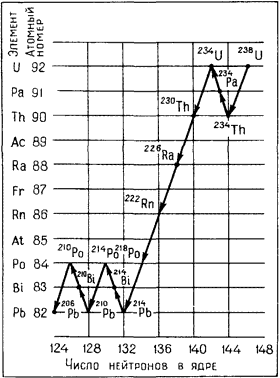
\includegraphics[width=0.48\textwidth]{pic1}
\halfspacing
\caption{Основная цепь радиоактивных превращений урана. По оси абсцисс отложено число нейтронов в ядре, а по оси ординат — число протонов (атомный номер элемента). Стрелки, направленные вниз, соответствуют процессу $\alpha$-распада. В этом процессе атомное ядро испускает быстрое ядро гелия ($\alpha$-частицу), теряя два протона и два нейтрона. Стрелки, направленные вверх, обозначают $\beta$-распад. В этом процессе ядерный нейтрон становится протоном и атомный номер увеличивается на единицу.}
\label{fig:example_figure}
\end{figure}
\fontsize{13.2}{15}\selectfont
ного для измерения сроков порядка миллиардов лет, должен быть такого же порядка величины. Лишь при этом условии радиоактивные атомы сохраняются в минерале до наших дней.

Первый процесс радиоактивного распада, который был использован для определения возраста минералов, — превращение изотопов урана в свинец.

Природный уран состоит из трех сортов атомов разной массы — изотопов 
$\ce{^{238}U}$, 
$\ce{^{235}U}$ и 
$\ce{^{234}U}$. Самый распространенный изотоп урана — 
$\ce{^{238}U}$. В уране, выделенном из любой горной породы, на его долю приходится 99,3\%.

Проследим за цепью радиоактивных превращений изотопа 
$\ce{^{238}U}$
(рис.1). Атомы
$\ce{^{238}_{92}U}$
медленно превращаются в атомы свинца (
$\ce{^{206}_{82}Pb}$
) и гелия (
$\ce{^{4}_{2}He}$
). Требуется 4,5 миллиарда лет, чтобы половина первоначального количества 
$\ce{^{238}_{92}U}$
перешла в свинец и гелий. Весь процесс включает 14 радиоактивных превращений, и в итоге каждый распавшийся атом урана даёт один атом стабильного свинца и восемь атомов гелия:

\[
\ce{^{238}_{92}U} \longrightarrow 8\ce{^{4}_{2}He} + \ce{^{206}_{82}Pb} + 6\ce{^{0}_{-1}e}.
\]

Возраст гранита можно определить следующим образом. Если кусок плотной породы, например гранита, размолоть в порошок, растворить его в кислоте, выделить из раствора свинец и уран, а затем найти соотношение количества атомов изотопа 
$\ce{^{206}_{82}Pb}$  к количеству атомов $\ce{^{238}_{92}U}$
, то по этим данным вычисляется возраст породы. Обозначим через $N$ число атомов урана, а через $N_1$ число атомов свинца $\ce{^{206}_{82}Pb}$
, содержащихся в минерале на момент анализа. Тогда 
$N_0 = N + N_1$
— это количество атомов урана в момент образования гранита. (Предполагается, что весь свинец в граните образовался из урана в результате радиоактивного распада.) Согласно закону радиоактивного распада:

\[
\frac{N}{N_0} = \frac{N}{N+N_1} = \left(\frac{1}{2}\right)^{\frac{t}{T_{1/2}}},
\]

где $t$ — возраст гранита, а $T_{1/2}$ — период полураспада урана-238.

Логарифмируя это равенство, получаем формулу для вычисления возраста минерала:

\[
t = \frac{T_{1/2}}{\ln 2} \ln \frac{N}{N_0}.
\]

При расчётах предполагается, что в образце отсутствует посторонний свинец и исключён обмен веществом с внешней средой. Однако это не всегда выполняется. Один из промежуточных продуктов в цепочке превращений урана в свинец является благородным газом (радон), и если изучаемый минерал недостаточно плотен, радон может улетучиться. В таком случае количество атомов свинца в образце окажется меньше, чем количество атомов урана, рас-
\newpage
павшихся за время существования
образца. При этом условии возраст
минерала, вычисленный по формуле (1), будет меньше действительного.
С другой стороны, в породе может
находиться свинец, появившийся одновременно с другими элементами
и попавший в минерал во время образования твердой земной коры. Такой свинец называют первичным. Наличие первичного свинца приводит
к завышению возраста горной породы. Поэтому для правильного определения возраста необходимо убедиться в том, что из минерала не
утекал радон, и уметь определить
долю первичного свинца в породе.
Свинец радиоактивного происхождения (радиогенный свинец) накапливается не только после распада изотопа $\ce{^{238}U}$, но образуется и в результате радиоактивных превращений
$\ce{^{235}U}$ и $\ce{^{232}Th}$. Изотоп $\ce{^{206}Pb}$ — потомок $\ce{^{238}U}$, а изотопы $\ce{^{207}Pb}$ и $\ce{^{208}Pb}$
замыкают цепь распада $\ce{^{235}U}$ и $\ce{^{232}Th}$
соответственно.
В природном свинце содержится
также легкий изотоп $\ce{^{201}Pb}$, который
не накапливается в цепях радиоактивных превращений ни одного из
природных радиоактивных элементов. Откуда взялся «легкий» свинец? Ответ один — свинец с массовым числом 204 образовался одновременно с другими элементами на
Земле.
Изотопный состав свинца без
радиогенных примесей был определен при анализе железных метеоритов. В таких метеоритах нет урана
и тория — источников радиогенного
свинца. Метеоритный свинец на одну
часть изотопа $\ce{^{204}Pb}$ содержит 10 частей $\ce{^{206}Pb}$, 10 частей $\ce{^{207}Pb}$ и 29 частей $\ce{^{208}Pb}$.
Изотопный анализ позволяет по
количеству изотопа $\ce{^{204}Pb}$ оценить количество первичного свинца в горной породе. Так, если в свинце
отсутствует изотоп $\ce{^{204}Pb}$ или содержится небольшая доля его, то
практически весь свинец радиогенного
происхождения.
Первые измерения возраста минералов и Земли радиоактивными методами дали значительно меньшие
значения, чем принятые в наши дни.
Ошибки, по-видимому, вкрадывались
из-за диффузии радона.
В дальнейшем были получены более точные значения возраста не только благодаря совершенствованию
свинцово-уранового метода, но и
за счет развития других способов.
Данные считаются вполне надежными,
когда ответы, полученные разными
путями, совпадают. К счастью, изотопы урана — не единственный набор атомных ядер с периодом полураспада, соизмеримым с длительностью геологических эр. В таблице
приведены другие радиоактивные
изотопы, позволяющие осуществлять
взаимную проверку возраста минералов.
В природном калии в небольших
количествах содержится радиоактивный изотоп $\ce{^{40}K}$ с периодом полураспада 1,3 миллиарда лет. Обычно
ядро $\ce{^{40}K}$ испускает электрон и пре-
\end{multicols}
\begin{table}[h!] % Плавающее окружение
    \doublespacing
    \centering % Центрирование таблицы
    \caption{} % Подпись
    \begin{tabular}{|l|c|c|} % Спецификация: 3 столбца, линии
        \hline
        Название метода (изотоп) & Измеряемый возраст (лет) & Период полураспада (лет) \\
        \hline
        Радиоуглеродный $\ce{^{14}С}$ & От 100 до 50 тысяч & 5570 \\
        \hline
        Калиево-аргонный $\ce{^{40}K}$ & Свыше 100 тысяч & 1,3*10^9 \\
        \hline
         Рубидиево-стронциевый $\ce{^{87}Rb}$ & Свыше 5 миллионов & 5,0*10^{10}\\
        \hline
        Свинцово-урановый $\ce{^{238}U}$ & Свыше 200 миллионов & 4,5*10^9 \\
        \hline
    \end{tabular}
\end{table}
\newpage
\end{document}